% -----------------------
%        PACKAGES
% -----------------------

\documentclass[12pt]{article}
\usepackage[english]{babel}
\usepackage[utf8x]{inputenc}
\usepackage{amsmath}
\usepackage{graphicx}
\usepackage[colorinlistoftodos]{todonotes}
\usepackage{geometry}

\begin{document}


% -----------------------
%       TITLE PAGE
% -----------------------

\begin{titlepage}
\center

% -----------------------
%       UNIVERSITY
% -----------------------

\textsc{\LARGE Politenico di Milano}\\[1cm]
\textsc{\Large Dipartimento di Elettronica, Informazione e Bioingegneria}\\[0.5cm]
\textsc{\large \textbf{Advanced Operating Systems:} Project Report}\\[1.5cm]

% -----------------------
%         TITLE
% -----------------------

\rule{\linewidth}{0.5mm} \\[0.4cm]
\vspace*{10pt}
{ \huge \bfseries Embedded Neural Network}\\[0.4cm]
\rule{\linewidth}{0.5mm} \\[1.5cm]

% -----------------------
%        AUTHORS
% -----------------------

\begin{minipage}[t]{0.4\textwidth}
\begin{flushleft} \large
\emph{Authors:}\\
Marina \textsc{Nikolic}\\
Michele \textsc{Scuttari}
\end{flushleft}
\end{minipage}
~
\begin{minipage}[t]{0.4\textwidth}
\begin{flushright} \large
\emph{Supervisor:} \\
Dr. Federico \textsc{Terraneo}
\end{flushright}
\end{minipage}\\[1.5cm]

% -----------------------
%          DATE
% -----------------------

{\large September 2019}\\[1.5cm]

% -----------------------
%	       LOGO
% -----------------------

\begin{center}
	
\includegraphics[scale=0.24]{img/Logo_Politecnico_Milano.png}                                               
\end{center}

\vfill

\end{titlepage}

% -----------------------
%        CHAPTERS
% -----------------------

\newgeometry{a4paper,top=2cm,bottom=2cm,left=2cm,right=2cm,heightrounded,bindingoffset=5mm}

\section{Introduction}

\subsection{The Problem To Solve}
The goal of this project is the recognition of specific sounds (whistles and hands claps) through the usage of a STM32 board and a neural network, deployed on the aformentioned board and acting as sound classifier.

\subsection{Why Neural Networks?}
For recognition and analysis of sound, AI techinques are used because of the complexity of the computations and the amount of noise present in the environment. Another important issue is that instances of the same sound have high variability due to different (yet homogeneous) sources. For example, think about words recognition: an effective application should recognise a word even if spoken by different people.

\subsubsection{Which kind of NN?}
The neural network used in this project is a sequential feed-forward one. Since the aim is to distinguish two different sounds, the NN is a classifier which input is the FFT of a time window and the output has one-hot encoding.\\
This simple model is expected to work because of the simplicity of the problem and the characterization of the two sounds.

\subsubsection{How to implement NN on a board?}
The \textbf{STM32cube.ai} allows to compile a pre-trained neural network into a library to be called in the code.

\subsection{Acronyms and Definitions}
\begin{itemize}
 \item \textbf{AI:} Artificial Intelligence
 \item \textbf{NN:} Neural Network
 \item \textbf{FFT:} Fast Fourier Transformation
\end{itemize}


\section{Design and Implementation}
\subsection{Board Programming}
\subsubsection{Board description}
The board in use is a \textbf{STM32F4 Discovery} (STM32F407VGT6) and is equipped with the open source operating system Miosix.\\
The peripherals used in this project are the microphone, the user button and the \text{USART}, although also the CRC module is enabled because needed by the ST's AI library.

\subsubsection{Microphone}
The board is equipped with a \textbf{MP45DT02} MEMS microphone, which produces a stream of 1-bit \textbf{Digital Pulse Modulation} (PDM) samples. The PDM samples are received using DMA and then converted to 16-bit signed \textbf{Pulse Code Modulation} (PCM) samples through the usage of a software low pass filter.\\
The PCM data is sampled at a frequency of 32 kHz, which is obtained by setting the \textit{PLLI2SN}, \textit{PLLI2SR} and \textit{I2SDIV} registers to appropriate values (see chapters \textit{7.3.23} and \textit{28.4.4} of the datasheet for further details):
\begin{flalign*}
&f_\text{(VCO clock)} = f_\text{(PLLI2S clock input)} * \frac{PLLI2SN}{PLLM} = 8\text{ MHz}\ \frac{213}{8} = 213 \text{ MHz}\\
&f_\text{(PLL I2S clock output)} = \frac{f_\text{(VCO clock)}}{PLLI2SR} = \frac{213\text{ MHz}}{2} = 106,5\text{ MHz}\\
&f_\text{(PDM)} = \frac{f_\text{(PLL I2S clock output)}}{2 * I2SDIV * 8} = \frac{106,5\text{ MHz}}{2 * 13 * 8} = 512\text{ kHz}\\
&f_\text{(PCM)} = \frac{f_\text{(PDM)}}{16} = \frac{512\text{ kHz}}{16} = 32\text{ kHz}
\end{flalign*}
The driver also uses a double buffering strategy: one buffer (the ``ready buffer'') contains the stable data that are sent to the network, while the other one (the ``processing buffer'') is populated by the new incoming samples. When the processing buffer is full, they are swapped and thus the meanwhile collected data becomes ready.
\begin{center}
    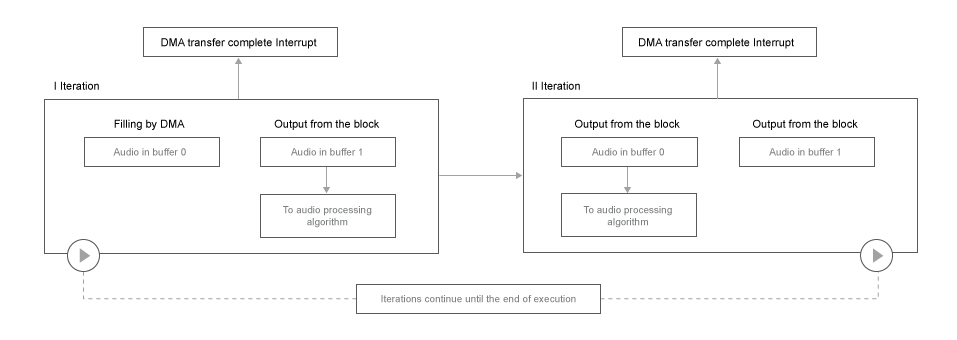
\includegraphics[width=\textwidth]{img/double_buffering_audio_in.png}
\end{center}

\subsubsection{FFT}
The PCM samples are considered in blocks of 1024 values, called ``windows''. Before the values are processed, they are normalized and passed through a \textbf{Hann function}, which makes sure that the discontinuity at the windows borders are eliminated. Then the FFT is computed and, being the output symmetric (because all the input has zero imaginary part), only half of the 1024 output bins are taken. Finally, the magnitude is computed on each single value.\\
Being the Cortex M4 equipped with the \textbf{Digital Signal Processor} (DSP), the FFTs are determined using the dedicated hardware.

\subsubsection{User button}
The user button press is handled by enabling the \textbf{EXTI0} interrupt.\\
The calling thread is paused while waiting for the press event, in order to allow other tasks to be executed meanwhile.\\
Moreover, a software debouncing feature is implemented in order to avoid multiple clicks due to the mechanical structure of the button. This is achieved is by recognizing the first button press and ignoring further clicks for a predefined amount of time (200 ms), whose length is sufficiently long to discard false clicks and small enough to improbably ignore real clicks.

\subsubsection{USART}
The communication between the board and the client is done through \text{USART} connection (\textit{PA2 = TX, PA3 = RX}), configured with a speed of \text{115200 bps}. The communication is set in raw mode by disabling the canonical mode and not converting controls (i.e. \textit{\^{}C}, \textit{\^{}Z}) into signals.

\subsubsection{Neural network library}
The neural network library is generated by the \textbf{X-CUBE-AI} expansion pack for STM32CubeMX. This tool automatically converts the pretrained Keras model into a C library that can be called by the main program.\\
Instead, the core of the network runtime is provided by ST as a static closed source library (\textit{neural\_network.a}).

\subsubsection{Issues}
\begin{itemize}
    \item The suggested IDE Netbeans gives a lot of troubles in the development, such as missing code completion and unrecognized definitions. So the Miosix build system has been converted to CMake, in order to allow the usage of modern IDEs such as CLion.
    \item The Miosix toolchain has a bug in the linking phase, resulting in the network runtime library to block in an infinite loop when its functions are called. To solve this issue, the linking process has been executed using the standard ARM linker.
\end{itemize}

\subsection{Network Training}
The software can be compiled in two different ways, by enabling or disabling the \textit{TRAINING} variable definition. When the variable is defined, the neural network is not executed and the FFT samples are directly transferred to the client. This way, it is possible to obtain the data to separately train the network. When the network is trained and uploaded, the variable definition can be removed in order to enable the normal operating mode, in which the neural network runs and outputs the recognized sounds.

\subsection{Testing}

\section{Experimental Results}

\section{Conclusions}
\subsection{...}
\subsection{Possible Use Cases}
\subsection{Future Improvements}


% delete when finished writing
\section{Some \LaTeX{} Examples}
\label{sec:examples}

\subsection{Sections}

Use section and subsection commands to organize your document. \LaTeX{} handles all the formatting and numbering automatically. Use ref and label commands for cross-references.

\subsection{Comments}

Comments can be added to the margins of the document using the \todo{Here's a comment in the margin!} todo command, as shown in the example on the right. You can also add inline comments too:

\todo[inline, color=green!40]{This is an inline comment.}

\subsection{Tables and Figures}

Use the table and tabular commands for basic tables --- see Table~\ref{tab:widgets}, for example. You can upload a figure (JPEG, PNG or PDF) using the files menu. To include it in your document, use the includegraphics command as in the code for Figure~\ref{fig:frog} below.

% Commands to include a figure:
\begin{figure}
\centering
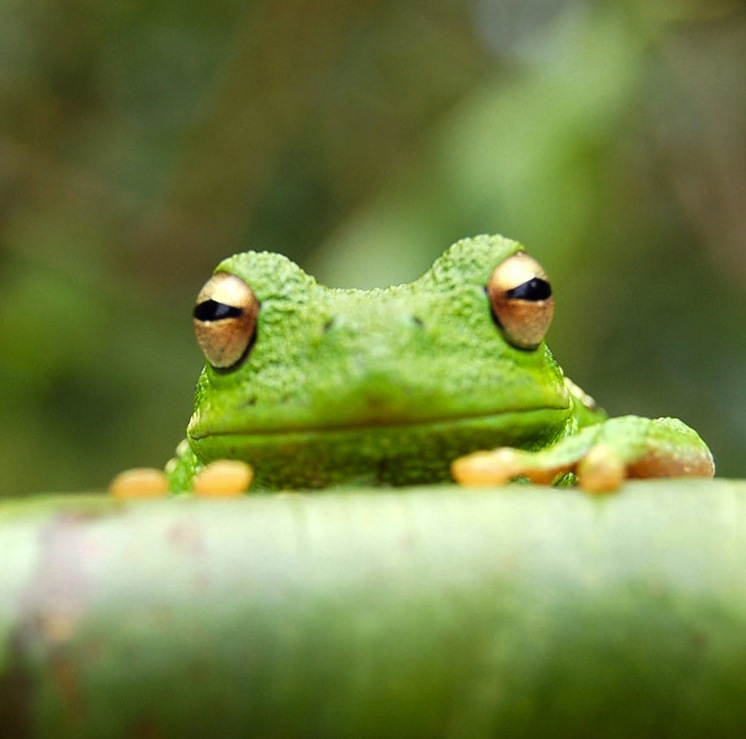
\includegraphics[width=0.5\textwidth]{frog.jpg}
\caption{\label{fig:frog}This is a figure caption.}
\end{figure}

\begin{table}
\centering
\begin{tabular}{l|r}
Item & Quantity \\\hline
Widgets & 42 \\
Gadgets & 13
\end{tabular}
\caption{\label{tab:widgets}An example table.}
\end{table}

\subsection{Mathematics}

\LaTeX{} is great at typesetting mathematics. Let $X_1, X_2, \ldots, X_n$ be a sequence of independent and identically distributed random variables with $\text{E}[X_i] = \mu$ and $\text{Var}[X_i] = \sigma^2 < \infty$, and let
$$S_n = \frac{X_1 + X_2 + \cdots + X_n}{n}
      = \frac{1}{n}\sum_{i}^{n} X_i$$
denote their mean. Then as $n$ approaches infinity, the random variables $\sqrt{n}(S_n - \mu)$ converge in distribution to a normal $\mathcal{N}(0, \sigma^2)$.

\subsection{Lists}

You can make lists with automatic numbering \dots

\begin{enumerate}
\item Like this,
\item and like this.
\end{enumerate}
\dots or bullet points \dots
\begin{itemize}
\item Like this,
\item and like this.
\end{itemize}

We hope you find write\LaTeX\ useful, and please let us know if you have any feedback using the help menu above.

\end{document}
